% !TEX root = ../literature.tex
\subsection{Summary}
Many researchers spend time and effort to explore how large displays can improve people's experiences. 
With the shift from private to public settings the explored solutions changed. 
It was highly impractical to put wires on people who wanted to use an installation naturally in a public environment [9].
With this limitation came different approaches for solving it. 
We identified two different areas which deals with it, we present them in \Cref{fig:litreview}.

\begin{figure*}
\centering
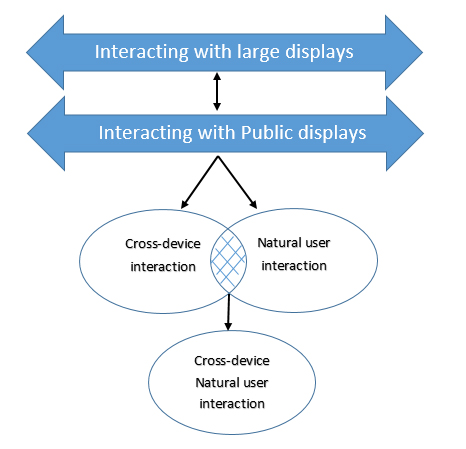
\epsfig{file=images/litreview-fig1.jpg, width=0.5\textwidth}
\caption{\todo{Write caption}}
\label{fig:litreview}
\end{figure*}
 \\
 
The fields of natural user interactions and cross-device interactions were thoroughly examined. 
We were surprised to see that research in combining features from the two areas is slim even though they are complementary to each other. 
There was research that was done [26, 27, 28, 29]. 
Interaction-techniques were evaluated with 3-6 people using qualitative surveys in [27,28,29] and without qualitative surveys in [26].\\

In summary, we can see research opportunities in further exploration of cross-device natural user interactions technique for large displays. 
Firstly, as handheld devices become thinner and lighter and spatially-aware technologies, such as Kinect, continue to evolve, this opens a potentially rich space of aforementioned techniques. 
Secondly, we see opportunities in quantitative aspect, for example comparative study of different interaction techniques. 
